%第4章:検証
%結果(実験で起こったこと)を書く.客観的に.グラフあればなおよし.


\section{検証}

本節では設計に対して行った検証の方法,結果について述べる.

\subsection{単体テスト}

詳細設計の際に作成した単体テストの項目に従い,単体テストを実施した.
単体テストの結果を表\ref{res_tantai}に示す.
\begin{table}[htbp]
    \centering
    \caption{センサデバイスを用いた単体テストの結果}
    \label{res_tantai}
    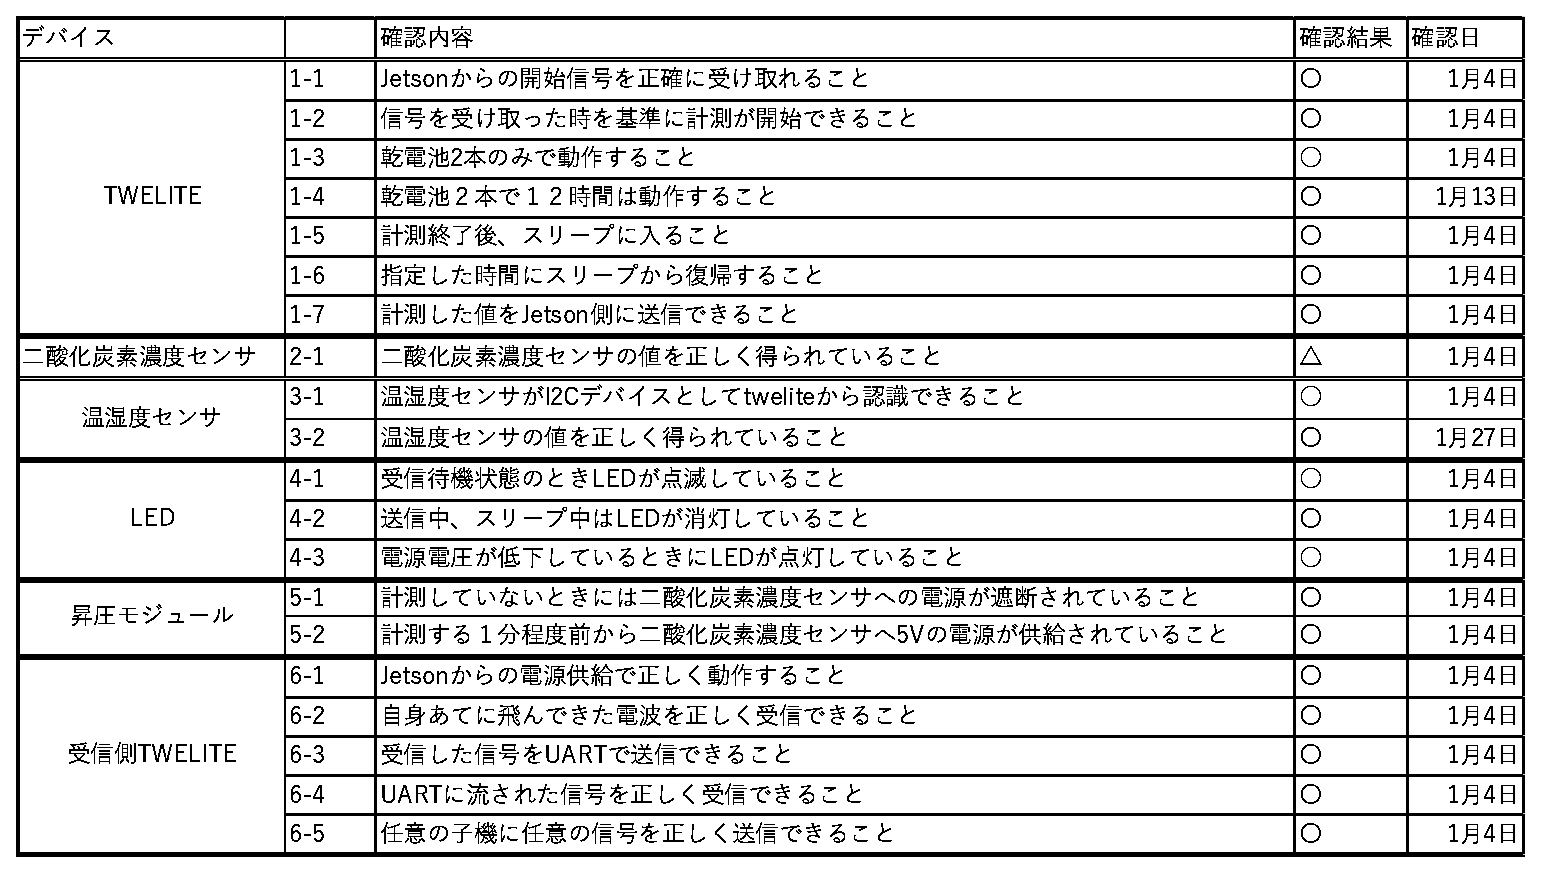
\includegraphics[width = 15cm]{./picture/tantaitest_twelite_kekka.eps}
\end{table}

検証方法および結果について詳しく述べる.
単体テスト実施においては,センサデバイスの詳細な動作を確認するため,TWELITEのUART接続を用い,デバイスをPCに接続した上で行った.
センサデバイス上で動くプログラムの中で随時UART出力を行い,その内容をPCの画面上で確認する方法を用いた.

項目1-1については,受信側TWELITEに対し開始信号を送る指示を出すことにより検証した.
TWELITEが受信した内容をPCの画面上で確認したところ,受信側TWELITEから送った信号が正しく受信できていることを確認した.
項目1-2については,状態遷移の際にUART出力を行うことで検証した.
受信側TWELITEからの電波を受信したときに,同時に「接続指示待機」状態から「センサヒートアップ待ち」状態へ遷移していることを確認した.
同様にして,項目1-5,項目1-6も検証し,正しく動作していることを確認した.
項目1-3については,単3型のアルカリ乾電池を2本電源として接続したときに,UART上で正常に起動メッセージが流れていることを確認し,正しく起動されていることを確認した.
項目1-4については,直接検証することが難しかったため,後述する消費電力の計測において満たしていることを確認した.
%項目1-4については,単3型のアルカリ乾電池2本を電源として用い,受信側TWELITEで受信した信号を記録することによって検証を行った.
%後で訂正
%約29時間41分間分が正常に記録されていたため,12時間以上動作していることが確認できた.
項目1-7については,センサデバイスを接続したPCの画面上で値を確認し,その後受信側TWELITEで受信した値と比較して,違いがないことを確認した.
項目2-1については,UART接続によってTWELITEが二酸化炭素濃度センサから取得した値を確認することで検証を行った.
窓をすべて開け,しばらく放置した部屋において平均で402ppmの値が観測でき,二酸化炭素濃度の2018年平均値である412ppm\cite{co2_ave}とほぼ同じ値が確認できた.
しかしながら,長時間経過後,時折観測上限値である5000ppm以上の値を観測することがあった.
電池の消耗による電源供給能力の不足であると考えられるが,これより評価を△とした.
また,これを受け,電源電圧低下を知らせるLEDの点灯の基準となる電圧を当初予定したTWELITEの最低必要電圧よりも高い値とすることで対処を行った.
さらに,使用電源も単4形よりも電気容量の多い単3形,そして比較的高電流用途に用いるアルカリ電池を必ず使用するようにした.
項目3-1については,$I^2C$でTWELITEが認識できたアドレス番地を確認し,それが温湿度センサのものと一致していることで確認を行った.
項目3-2については,$I^2C$を介して得られた値を確認することで検証を行った.
温度については別のデジタル温度計による観測値が$19.1 ^\circ C$である環境の中で,$18.86^\circ C$の値を取得していた.
また,湿度の値については気象庁による同市,同時間の観測データ\cite{amedas}が52\%であったときに%45.08\%
55.54\%の値を取得していた.
これらの値はBME280の測定精度が温度$\pm{1}^\circ C$,湿度$\pm{3}\%$であることより,おおむねこの範囲程度の値が観測されていたため,〇とした.
項目4-1については,状態遷移した記録をもとに現在の状態を導き,その時のLEDの状態を観測することで検証した.
同様に,項目4-2についても検証を行い,うまく動作していることを確認した.
項目4-3については,起電力の低い充電式の電池を用い,受信待機状態から推移したのちにLEDが点灯したままであることを確認した.
項目5-1については,昇圧モジュールの端子部分にテスターを当て,電源が供給されているかどうかを確認した.
項目5-2についても同様に行い,設計通りの動作ができていることを確認した.
項目6-1については,JetsonのGPIO端子に接続し,TWELITEに対して正常に送受信が行えていることを確認した.
項目6-2については,受信側TWELITEをUART接続によりPCと接続し,PCの画面上で受信された情報を確認することで検証を行った.
TWELITEで観測された値と受信した情報が一致していることを確認した.
同様にPCよりUART接続を行い,項目6-3,項目6-4,項目6-5についても満たしていることを確認した.

\subsection*{消費電力の計測}
センサデバイスの連続稼働時間を求めるため,実際の消費電力の計測を行った.
消費電力は電圧値と電流値によって計算されるが,同時に計測することが難しいため,電圧は3.0Vで固定であるとし,電流を計測することでそれに変えることとした.
電流の計測においては,図\ref{keisoku_kairozu}に示すように,電源の+極から流れる電流を計測することでこれを実施した.
なお,本計測においては,実際の使用の際の正確な消費電力を計測するため,UART接続でのPCへの接続は行わなかった.
\begin{figure}[htbp]
    \centering
    \includegraphics[width = 15cm]{./picture/kairozu_keisoku.eps}
    \caption{センサデバイスの電流測定の際の回路図}
    \label{keisoku_kairozu}
\end{figure}

まず,「接続指示待機」状態については,電源を接続し,受信側TWELITEから電波を送信しない状態で放置し,その時の電流値を測定した.
測定は9分間行い,0.25秒おきに電流値の取得を行い,平均値を求めたところ,60mAとなった.
続いて,「時間待ち」,「センサ読み取り」,「センサヒートアップ待ち」状態については,外部から状態推移を確認できなかったため,受信側TWELITEより開始信号を送り,受信待機状態を示すLEDが消灯してからしばらくの間の電流値を測定した.
測定を12分間,0.25秒おきに電流値の取得を行った.
3分ごとにこれらの状態の推移が完了しているため,結果を3分ごとに区切り,4サイクル分としてそれぞれの時間における平均電流値を求めた.
その変化を図\ref{tuujou_denryoku}に示す.
\begin{figure}[htbp]
    \centering
    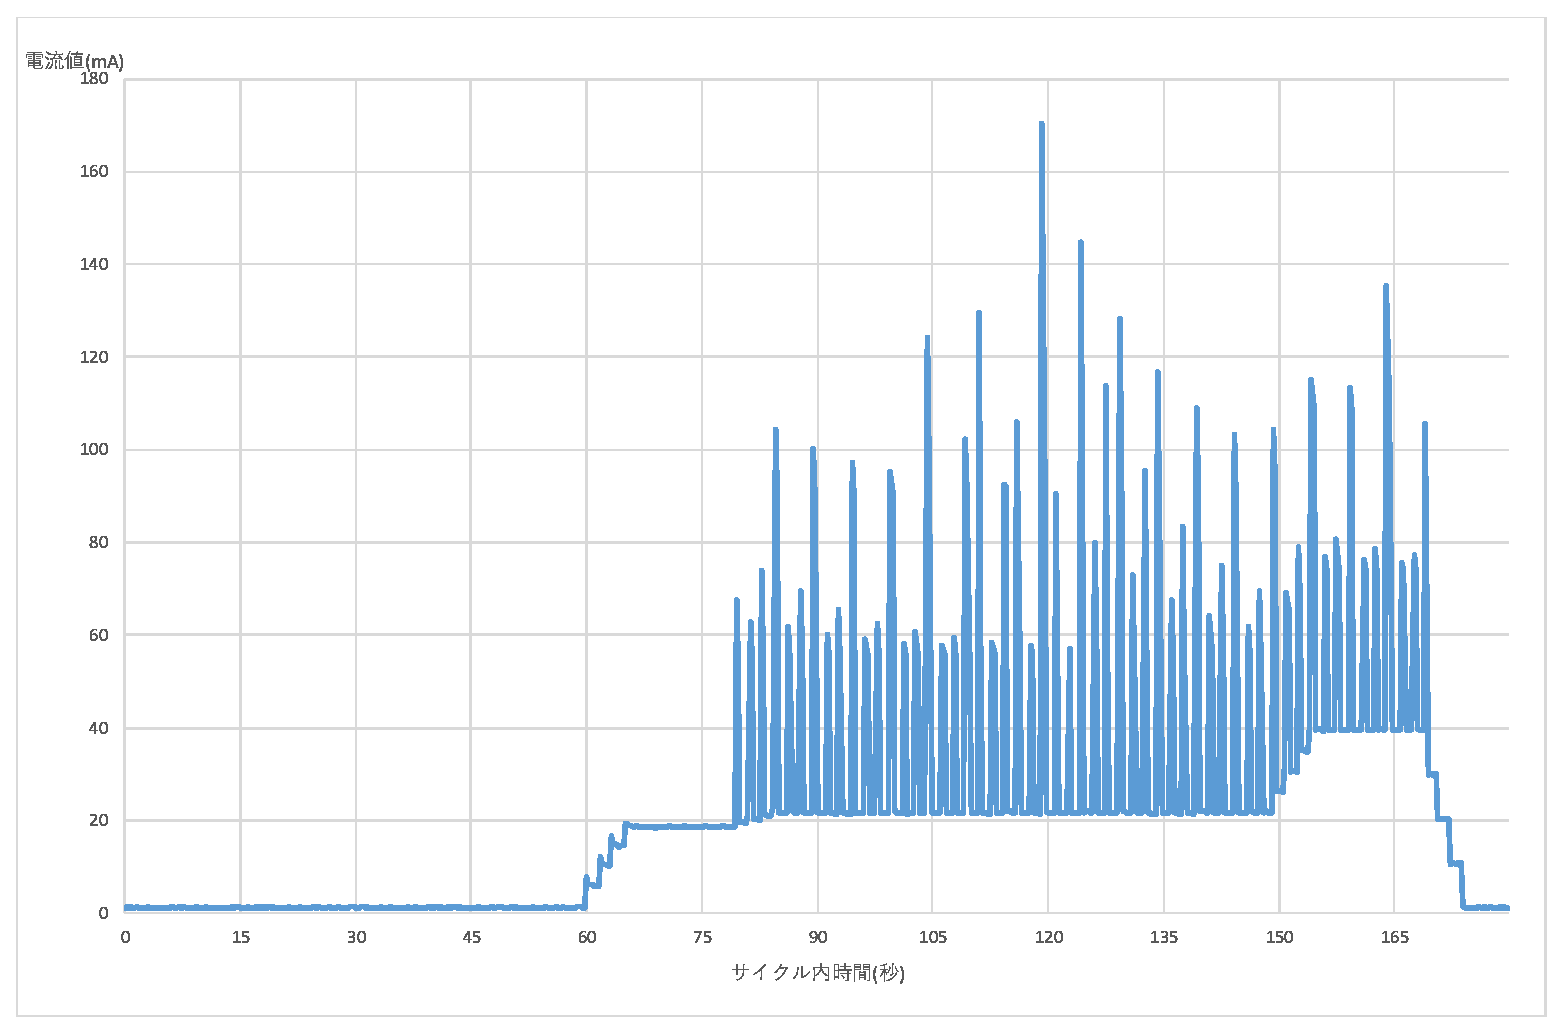
\includegraphics[width = 15cm]{./picture/tuujou_dennryoku.eps}
    \caption{観測された平均電力値の推移}
    \label{tuujou_denryoku}
\end{figure}
この結果より,特に比較的長時間電流が低い状態となっている,0秒から60秒までの範囲が「時間待ち」状態であったと推定して,その平均値を求めたところ,1.2mAとなった.
また,150秒から165秒においては比較的電流が高い状態で推移しているため,「センサ読み取り」状態であったと推定して,その平均値を求めたところ,53mAであった.
それらの状態の間で,かつ消費電力が「センサ読み取り」状態よりは比較的電流が少ない状態となっている,75秒から135秒が「センサヒートアップ待ち」状態であったと推定して,その平均値を求めたところ,37mAであった.
最後に,受信側TWELITEによって開始信号を送ったのち,受信側TWELITEでセンサデバイスから発信される電波を監視し,10分間電波が監視されなかった後を「夜間スリープ」状態に入ったと推定して,その電流値を測定した.
測定は23分間,0.25秒おきに電流値の測定を行い,その平均値を求めたところ,1.2mAであった.

以上の結果を踏まえ,実装の際に行った見積りと同じように計算を行うと,1日当たりの消費電流は320mAhとなった.
単3型アルカリ電池2本で合計4000mAhの電池容量を持つとすると,12日以上連続して使用可能であるという計算になる.
以上のことより,単体テストの項目1-4は満たしていることを確認した.

% V字モデルに従い,詳細設計の要件を満たしているかどうかを確認する.まず,各種センサが要件を満たすか否かを検証した.次に,各種センサのテスト項目に従い,単体テストを行った.単体テストの第一段階として,確認内容の頭に*印のついていないテスト項目の機能テストを行った.*印のついているテスト項目についてはLEDの点灯に関するものであり,追加を優先する機能ではないと判断し,第二段階のテストに含めた.


% \subsection*{Webカメラ}


% Webカメラの単体テストを表\ref{t_web}に示す.


% \begin{table}[htbp]
% \centering
% \caption{Webカメラの単体テスト}
% \includegraphics[width = 15cm]{./picture/tantai_web.eps}
% \label{t_web}
% \end{table}

% まず,表\ref{webcamera}における項目1のテストを行った.対象商品をカメラから100mm,150mm,200mmと離し,バーコードを読み取りが可能か,テストをした.カゴの高さが240mmかつ,Webカメラの設置場所はカゴの上部否かを90mmのため,150~200mm程度までバーコードが認識できれば要件を満たすとする.

% はじめに,WebカメラとしてロジクールC270を使用し,テストを行った.しかしながら,全ての画像のピントが合っておらず,バーコードを読み取ることができなかった.より画質が高く,ピントの合いやすいスマートフォンのカメラで撮影した動画でバーコード読み取りを試したところ,100mm,150mm程度まで読み取ることができたため,バーコード読み取りシステムの不具合ではなかったことが判明した.画素数もしくはピントを合わせる機能が問題になっていると仮定した.

% 次に,Raspberry Pi カメラモジュール V2を使用し,テストを行った.Raspberry Pi カメラモジュール V2については画素数はロジクールC270の約6.6倍の画素数のため,もし画素数に問題があるならば判明すると考えた.Raspberry Pi カメラモジュール V2をテストしたところ,ロジクールC270と同じようにピントが合わず,バーコードを読み取ることができなかった.

% 画素の問題でないことが判明したため,オートフォーカスモデルのロジクールC615を使用しテストを行った.バーコードの読み取り距離について要求を満たしたため,表\ref{jissou}に最終的な実装環境として記載したとおり,ロジクールウェブカメラC615を実装環境とした.項目2においても要求を満たしたことを確認した.


% \subsection*{超音波センサ}

% 超音波センサの単体テストを表\ref{t_chou}に示す.


% \begin{table}[htbp]
% \centering
% \caption{超音波センサの単体テスト}
% \includegraphics[width = 15cm]{./picture/tantai_chou.eps}
% \label{t_chou}
% \end{table}

% 最初に,超音波センサが正しく反応しているか,要求を満たしているかテストを行った.要求としてはカゴの横幅360mmなので,360mm以内を10mm程ずつ測ることができるかどうか確認した.超音波センサは正しく反応し,360mm以上の距離を1mmより小さい距離ずつ測ることができ,要求を満たした.

% 次に,第一段階の機能テストを行い,機能項目を満たしたことを確認した.同様に,第二段階の機能テストを行い,機能項目を満たしたことを確認した.

% \subsection*{ロードセル}

% ロードセルの単体テストを表\ref{t_rodoseru}に示す.


% \begin{table}[htbp]
% \centering
% \caption{ロードセルの単体テスト}
% \includegraphics[width = 15cm]{./picture/tantai_rodo.eps}
% \label{t_rodoseru}
% \end{table}

% ロードセルが正しく反応しているか,要求を満たしているかテストを行った.要求として,重量の増減を確認できるか,3kgまでの重量を1g程ずつはかることができるかどうか確認した.ロードセルは正しく反応し,対象商品を1gより小さい値ずつ測ることができた.そのためロードセルは要求を満たした.


% \subsection*{データ送信}

% データ送信における単体テストを表\ref{t_data}に示す.


% \begin{table}[htbp]
% \centering
% \caption{データ送信の単体テスト}
% \includegraphics[width = 15cm]{./picture/tantai_data.eps}
% \label{t_data}
% \end{table}

% 第一段階の機能テストを行い,機能項目を満たしたことを確認した.同様に,第二段階の機能テストを行い,機能項目を満たしたことを確認した.


\subsection{結合テスト}
基本設計の際に作成した結合テストの項目に従い,結合テストを実施した.
結合テストの結果を表\ref{res_ketsugo}に示す.
\begin{table}[htbp]
    \centering
    \caption{結合テストの結果}
    \label{res_ketsugo}
    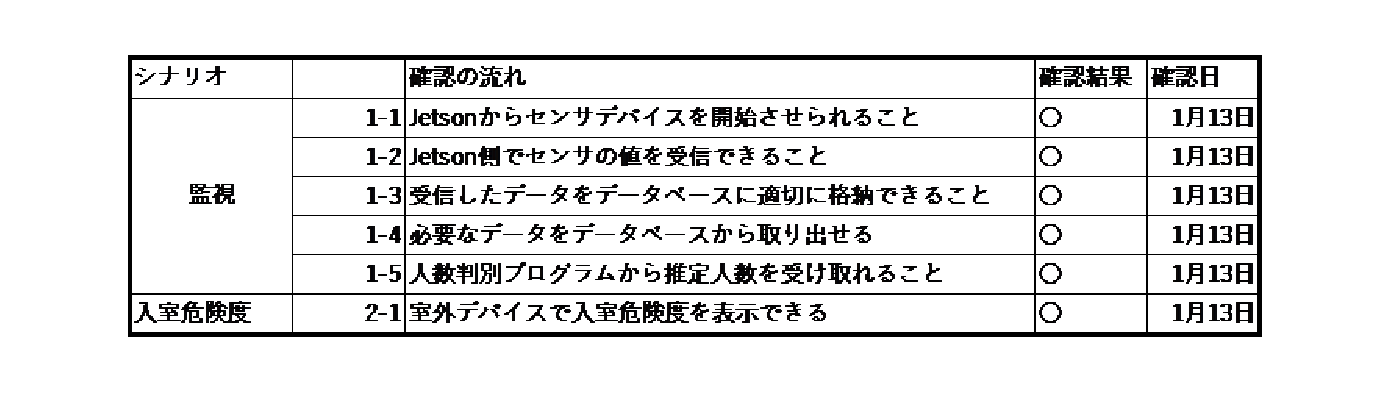
\includegraphics[width = 15cm]{./picture/ketugoutest.eps}
\end{table}

結合テストにおいては,環境値評価と人数推定を行う機能を同一プログラムで行えるようにした状態で行った.
また,データベースの処理も同一Jetsonで行えるようにし,受信用TWELITEをGPIO接続で接続した状態で行った.

項目1-1については,センサデバイスの電源を入れた状態でJetsonの処理プログラムを実行し,LEDの状態の変化によって状態推移が行われていることを確認した.
項目1-2については,Jetson上での処理プログラムを実行させることで,センサデバイスから電波が受信していることを確認した.
項目1-3については,処理プログラムの動作中にデータベースに格納された値を定期的に確認し,受信したデータが増えていることを確認した.
項目1-4については,データベースにデータが入っている状態で,その値を用いて評価が行えていることを確認した.
項目1-5については,処理の中心となるプログラムの中で,人数推定の結果を正しく入手出来ていることを確認した.
項目2-1については,Jetson上で評価を行った結果と,屋外デバイスのLEDの状態の変化を比較して検証した.
評価の結果に応じたLEDが正しく点灯していることを確認した.
% V字モデルに従い,基本設計の要件を満たしているか否かを確認する.各実装対象の結合テストを表\ref{t_ketsugo}に示す.


% \begin{table}[htbp]
% \centering
% \caption{結合テスト}
% \includegraphics[width = 15cm]{./picture/t_ketsugo.eps}
% \label{t_ketsugo}
% \end{table}

% 結合テストの際も,*印以外のテスト項目の機能テストを第一段階として行った.テスト項目14,15の画像をサーバに送信する際,Webカメラから撮影した画像とフラグをセットする順番について問題があった.超音波センサが反応するタイミングとロードセルが反応するタイミングが固定ではなく,どちらが先になるかが予想できなかった.画像とフラグをセットにしてデータを送信する際,画像が先に届くか,フラグが先に届くかが決まっている必要があったため画像とフラグをセットにする方法について考慮する必要があった.解決策として,フラグをキューへ追加し,画像撮影後,画像を画像用の配列へ追加,その後キューからフラグを取り出し,画像の後にフラグを入れセットにして送信する方法を採用した.画像を撮影後,キューが空の場合はフラグがたつまで一定時間待機することとした.上記方法で再度テストを行ったところ,正しく動作を確認した.

% 次に,*印を含める第二段階のテストを行った.テスト項目17のLEDの点滅について,点灯のほうがテストの際に確認がしやすかったため,項目17は点滅ではなく点灯として動作を確認した.テスト項目18においては,LED赤・青が誤作動し,複数回点灯することがあったため△とした.しかしながら,実際にユーザに正しく情報を伝えることができており,比較的優先度の低いテスト項目だったため,そのまま総合テストへ移行した.


\subsection{総合テスト}
要求定義の際に作成した総合テストの項目に従い,総合テストを実施した.
総合テストの結果を表\ref{res_sogo}に示す.
\begin{table}[htbp]
    \centering
    \caption{総合テストの結果}
    \label{res_sogo}
    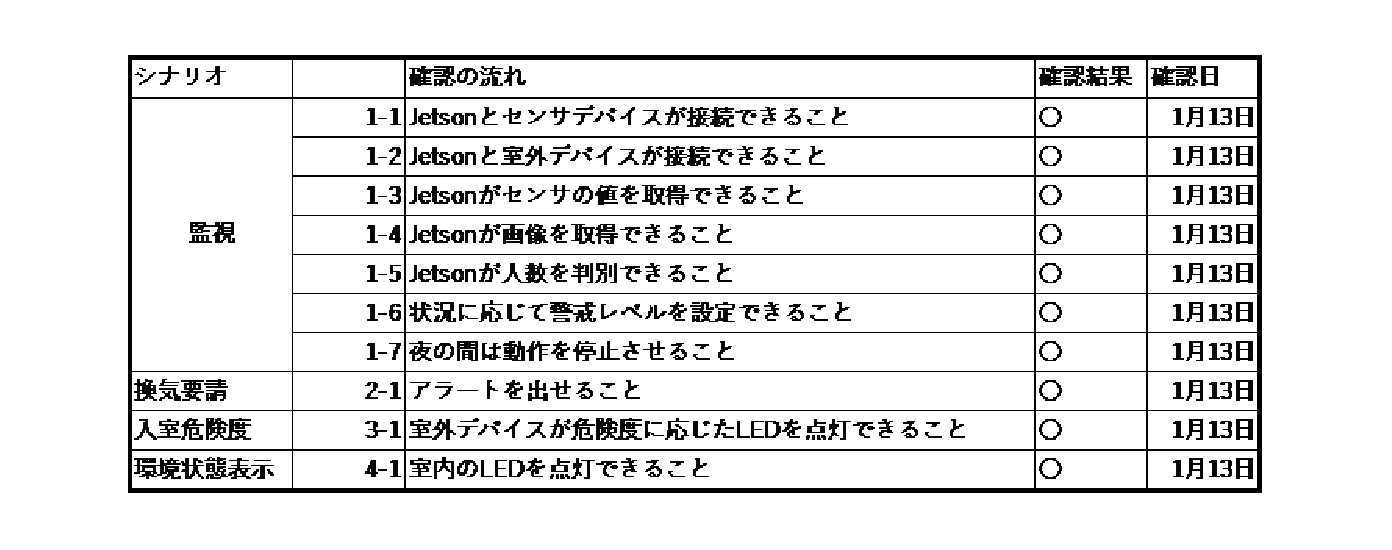
\includegraphics[width = 15cm]{./picture/sougoutest.eps}
\end{table}

総合テストは,実際のシステムの利用を想定し,各モジュールの接続を行い,センサデバイスを2台用いて行った.
各ユースケースの要求が満たされているかを確認した.

項目1-1においては,システム実行時に,センサデバイスがJetsonからの開始信号を受け取り,LEDの状態が変わっていることを確認した.
項目1-2においては,システム実行時に屋外デバイスのLEDが消灯状態になり,そこからJetsonからの指示のみでLEDの状態が変化できていることを確認した.
項目1-3においては,Jetsonがセンサデバイスから送信された値を受信でき,それを処理に利用できていることを確認した.
項目1-4については,Jetsonに接続されたWebカメラの画像をJetsonに接続した画面上で確認することによって検証を行った.
Webカメラからの画像が正しく取得されていることを確認した.
項目1-5については,人数が違う集合写真を用い,それぞれで人数推定が行えているかを確認した.
Webカメラに映った範囲において,おおむね正しく人数推定ができていることを確認した.
項目1-6においては,人数が多い写真を認識したときに,二酸化炭素濃度値が高いとにアラートを出し,警戒レベルが上がっていることを確認した.
同様に,項目2-1,項目3-1,項目4-1も確認し,アラート発生の際にJetsonに接続されたLED,ブザーが正しく機能していることを確認した.
項目1-7においては,人の出入りが少ない時間を設定し,その時間中,環境値収集,およびシステムの処理が中断されていることを確認した.

% V字モデルに従い,要求分析を満たしているかどうかを確認する.各実装対象のシナリオに基づいた総合テストを表\ref{t_sogo}に示す.


% \begin{table}[htbp]
% \centering
% \caption{総合テスト}
% \includegraphics[width = 15cm]{./picture/t_sogo.eps}
% \label{t_sogo}
% \end{table}

% 総合テストでは,3.1節の表\ref{sina}のシナリオに沿って動作しているかを確認する.テスト項目1-8においては,LED点灯の誤作動が度々あったため△とした.しかしながら,ユーザに通知するべき情報は正しく通知できていることを確認した.また,シナリオの流れも含め,表\ref{sogo}を確認した.
